% +--------------------------------------------------------------------+
% | Sample Chapter 3
% +--------------------------------------------------------------------+

\cleardoublepage

% +--------------------------------------------------------------------+
% | Replace "This is Chapter 3" below with the title of your chapter.
% | LaTeX will automatically number the chapters.
% +--------------------------------------------------------------------+

\chapter{Diseño de la aplicación}
\label{makereference3}

\section{Stakeholders}
\label{makereference3.1}

\section{Escenarios}
\label{makereference3.2}

\section{Requisitos funcionales}
\label{makereference3.3}

\section{Interfaz de usuario}
\label{makereference3.4}

\section{Sistema de recomendación}
\label{makereference3.5}

\section{Prototipos}
\label{makereference3.6}

\subsection{ARCore} 
\label{makereference3.6.1} 
 
\subsection{ViroMedia} 
\label{makereference3.6.2} 
 
\subsection{Vuforia + Android} 
\label{makereference3.6.3} 
 
En este prototipo utilizamos la librería nativa de Vuforia para Android para 
realizar las pruebas de tecnología de reconocimiento de imágenes tanto en  
local como usando la nube que nos ofrecía Vuforia, para la posterior renderización
de objetos y textos.

Las características tecnológicas de este prototipo son las siguientes:
\begin{enumerate}
    \item The first item
    \begin{enumerate}
    \item Nested item 1
    \item Nested item 2
    \end{enumerate}
    \item The second item
    \item The third etc \ldots
    \end{enumerate}
1. La librería de Vuforia para android está diseñada a muy baja nivel. 

2. Vuforia para dibujar en 3D usa la librería OpenGL.

3. OpenGL utiliza una serie de espacios donde se va colocando las cosas:

Local space: Es el espacio local de cada objeto.
World space: Es el mundo donde se encuentra los objetos.
View space: El mundo visto desde la perspectiva de la cámara.
Clip space: Se integra con la pantalla del móvil y definiendo los límites 
visibles, se establece unas coordenadas de rango -1.0 - 1.0

Las transformaciones de estos espacios se realiza mediante matrices 4x4 
el cual la primera fila significa el punto x, la segunda el punto y y la 
tercera z, mientras que la última columna significa los desplazamientos 
de los objetos de esos ejes.

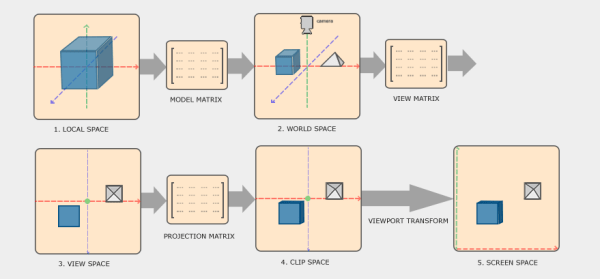
\includegraphics[height=2.5in]{figures/space-transformation.png}

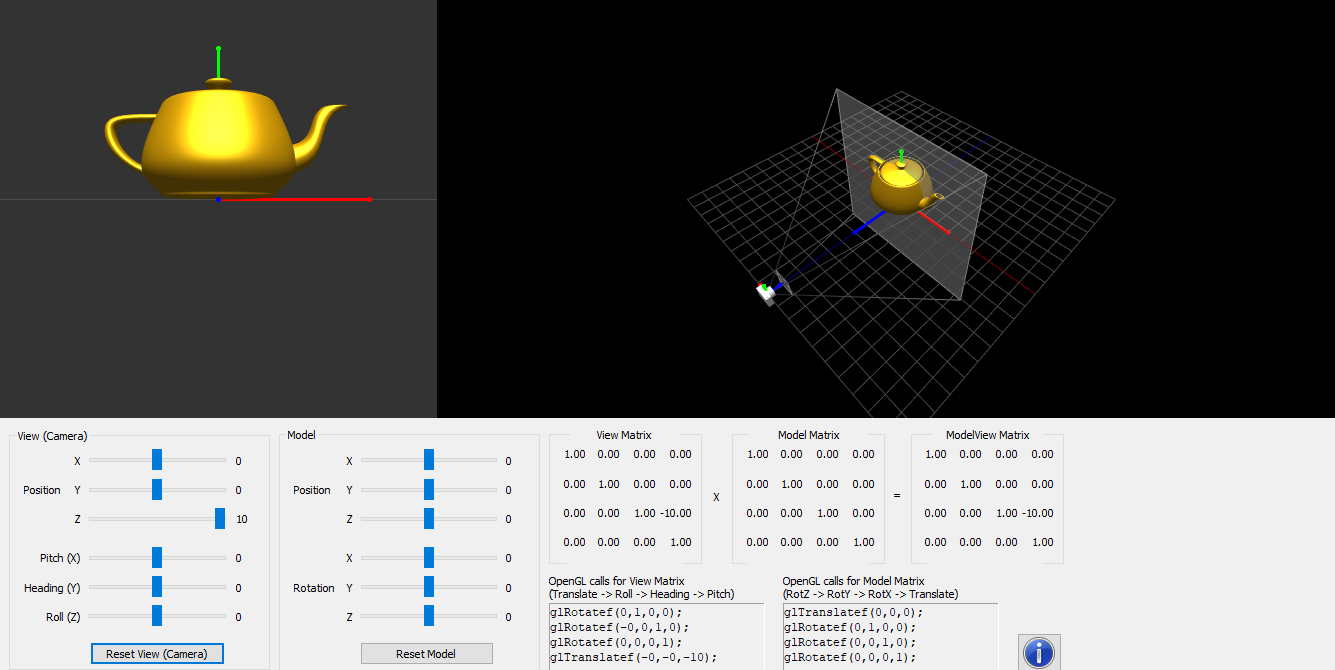
\includegraphics[height=2.5in]{figures/teapot.png}

3. En OpenGL es necesario escribir código para las tarjetas gráficas, el lenguaje que se usa es GLSL.
este código de GLSL se escribe en forma de String y se llama a un método 
que proporciona OpenGL.

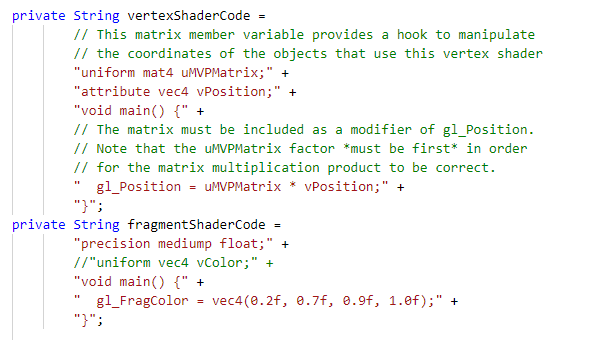
\includegraphics[height=2.5in]{figures/GLSL.png}

4. Otro aspecto es que OpenGL solo ofrece lo básico, no ofrece métodos para dibujar directamente objetos sino 
que hay que seguir un pipeline de procesos para conseguir dibujar algo.

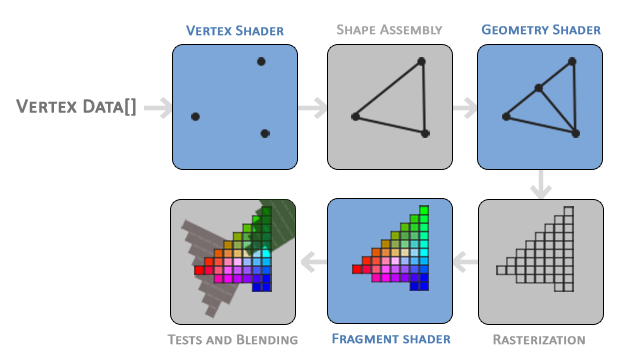
\includegraphics[height=2.5in]{figures/pipeline.png}

Esto consiste en pasar un array de números (cada tres para definir un punto) 
a las tarjetas gráficas, establecer triángulos entre los puntos (más array de números) 
definir colores a partir de los puntos (más arrays)..., y con el código del shader, ejecutar 
estos datos.

5. Por último como sólo ofrece métodos básicos, no hay métodos de escritura de texto, y la forma que 
encontramos y que funcione fue usar un bitmap con los caracteres.

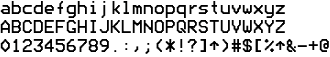
\includegraphics[height=2.5in]{figures/bitmap-font.png}

Rechazamos esto por un principal motivo, para hacer que funciones hay que codificar a muy bajo nivel y 
nos costaría mucho tiempo y esfuerzo.
 
\subsection{Vuforia + Unity} 
\label{makereference3.6.4}